\documentclass[12pt, a4paper]{article}

% ==========================================
% 1. CODIFICACIÓN Y TIPOGRAFÍA
% ==========================================
\usepackage[utf8]{inputenc}
\usepackage[T1]{fontenc}
\usepackage[spanish, es-tabla]{babel} % 'es-tabla' cambia "Cuadro" por "Tabla" automáticamente
\usepackage{amsmath, amssymb}         % Paquetes matemáticos antes de newtxmath
\usepackage{newtxtext, newtxmath}     % Tipografía Times New Roman (12pt según bases)
\usepackage{microtype}                % Mejora la justificación y estética tipográfica
\usepackage{amssymb}  % Para usar \checkmark
\usepackage{pifont}   % Opcional: para símbolos adicionales como cruces
\newcommand{\cmark}{\checkmark} % Check
\newcommand{\xmark}{\ding{55}}     % Cruz 
% ==========================================
% 2. MARGENES E INTERLINEADO (SEGÚN RÚBRICA)
% ==========================================
\usepackage[margin=2.5cm]{geometry}
\usepackage{setspace}
\onehalfspacing                       % Interlineado 1.5 obligatorio
\setlength{\parindent}{0.5cm}         % Sangría de 0.5 cm

% ==========================================
% 3. MATEMÁTICAS, UNIDADES Y TABLAS
% ==========================================
\usepackage{siunitx}                  % Para unidades físicas (ej. \SI{25}{\degree\Celsius})
\sisetup{output-decimal-marker = {,}}  % Coma decimal para español

\usepackage[table]{xcolor}            % Colores con soporte para tablas
\usepackage{booktabs}                 % Tablas profesionales (\toprule, \midrule, \bottomrule)
\usepackage{tabularx}
\usepackage{array}
\usepackage{makecell}
\usepackage{adjustbox}                % Ajuste de tablas anchas
\usepackage{multirow}                 % Necesario para combinar filas en la tabla
\usepackage{ragged2e}

% ==========================================
% 4. FIGURAS Y GRÁFICOS
% ==========================================
\usepackage{graphicx}
\graphicspath{{imagenes/}}
\usepackage{float}
\usepackage{caption}
\usepackage{subcaption}
\captionsetup{font=small, labelfont=bf, justification=centering}

\usepackage{tikz}
\usetikzlibrary{positioning, arrows.meta, babel}

% ==========================================
% 5. BIBLIOGRAFÍA (APA 7) Y ENLACES
% ==========================================
\usepackage{csquotes}
\usepackage[style=apa, backend=biber]{biblatex}
\addbibresource{referencias.bib}

\usepackage[colorlinks=true, linkcolor=black, urlcolor=black, citecolor=black]{hyperref}
\usepackage{bookmark}

% ==========================================
% 6. ENCABEZADOS Y PIE DE PÁGINA
% ==========================================
\usepackage{fancyhdr}
\pagestyle{fancy}
\setlength{\headheight}{15pt}
\fancyhf{}
\fancyhead[L]{\textbf{\coursename} (\coursecode)}
\fancyhead[R]{\small Entrega: \deliverydate}
\fancyfoot[C]{\thepage}
\renewcommand{\headrulewidth}{0.4pt}

% ==========================================
% 7. COMANDOS PERSONALIZADOS
% ==========================================
% Encabezados rotados a 90° para tablas estrechas
\newcommand{\rot}[1]{\rotatebox[origin=l]{90}{\parbox{2.8cm}{\raggedright #1}}}

% Marcador de contenido pendiente (eliminar antes de la entrega)
\newcommand{\pendiente}[1]{\textcolor{red}{[#1]}}

% ==========================================
% 8. DATOS DEL DOCUMENTO
% ==========================================
\newcommand{\univname}{Pontificia Universidad Católica de Chile}
\newcommand{\schoolname}{Escuela de Ingeniería}
\newcommand{\deptname}{Departamento de Ingeniería Mecánica y Metalúrgica}

\newcommand{\coursename}{Taller de Diseño de Productos Mecánicos}
\newcommand{\coursecode}{ICM3390}
\newcommand{\projecttitle}{Desafío 2: Acondicionador térmico de líquidos de sobremesa}

\newcommand{\authorone}{Juan Francisco Ruz Aedo}
\newcommand{\authortwo}{Francisco Joaquín Retamal Suárez}
\newcommand{\authorthree}{Nicolás Rodrigo Meyer Sironvalle}
\newcommand{\authorfour}{Adolfo Claudio Leiva Mendoza}

\newcommand{\deliverydate}{26 de octubre de 2026}

% ==========================================
% INICIO DEL DOCUMENTO
% ==========================================
\begin{document}

% ------------------------------------------
% PORTADA
% ------------------------------------------
\begin{titlepage}
    \centering
    
    % Logo de la Universidad (Asegúrate de tener 'logo-uc.jpg' en tu carpeta o carpeta imagenes/)
    
\includegraphics[width=0.2\textwidth]{logo-uc.jpg}\par
    \vspace{0.5cm}
    
    {\Large \scshape \univname \par}
    \vspace{0.2cm}
    {\large \scshape \schoolname \par}
    \vspace{0.1cm}
    {\normalsize \scshape \deptname \par}
    
    \vspace{0.5cm}
    \rule{\linewidth}{1pt} \par
    \vspace{0.5cm}

    {\Huge \bfseries \projecttitle \par}
    \vspace{0.3cm}
    {\Large Grupo 6 \par}
    \vspace{0.3cm}
    {\large \coursename{} -- \coursecode \par}
    
    \vspace{0.5cm}
    \rule{\linewidth}{1pt} \par

    \vfill 
    
    % Distribución de Integrantes y Docentes
    \begin{minipage}[t]{0.5\textwidth}
        \begin{flushleft} \large
            \textbf{Integrantes:} \\
            \authorone \\
            \authortwo \\
            \authorthree \\
            \authorfour
        \end{flushleft}
    \end{minipage}
    \hfill
    \begin{minipage}[t]{0.4\textwidth}
        \begin{flushright} \large
            \textbf{Profesores:} \\
            Juan Pablo Oyarzun Alcayaga \\
            Ariel Orlando Espinoza Jara
        \end{flushright}
    \end{minipage}

    \vspace{1.5cm}

    {\large \deliverydate \par}
\end{titlepage}

% --- CONFIGURACIÓN DE NUMERACIÓN DESDE EL ÍNDICE ---
\pagenumbering{arabic}
\setcounter{page}{1}

% ------------------------------------------
% ÍNDICES
% ------------------------------------------
\tableofcontents
\newpage
\listoffigures
\listoftables
\newpage

% ==============================================================================
% SECCIONES DEL INFORME (Estructura oficial exigida)
% ==============================================================================

\section{Introducción y contexto de uso}

\section{Necesidades, especificaciones y selección del concepto}
\subsection{Usuario}
Para dar inicio a la elaboración del desafío, se define como usuario a aquellas personas que requieran enfriar bebestibles individuales o calentar alimentos de pequeñas porciones en su hogar, oficina o lugar de estudio. Con el objetivo de conocer las prioridades de este grupo, se aplica una encuesta mediante un formulario en línea a 9 personas representativas del usuario definido.

\subsection{Necesidades}
A partir del análisis del contexto de uso y de los requerimientos del encargo, se identifican las siguientes necesidades del usuario:

\begin{enumerate}
    \item \textbf{Enfriamiento efectivo:} Alcanzar la temperatura ideal de consumo para latas de bebida.
    \item \textbf{Calentamiento efectivo:} Elevar el agua a la temperatura adecuada para la sopa.
    \item \textbf{Tiempo de respuesta:} Completar el acondicionamiento térmico en un rango de tiempo breve.
    \item \textbf{Facilidad de uso:} Operación simple e intuitiva para el usuario.
    \item \textbf{Limpieza e higiene:} Limpieza rápida y accesible de las piezas en contacto con alimentos.
    \item \textbf{Portabilidad:} Diseño compacto y transportable para entornos domésticos o de oficina.
    \item \textbf{Inocuidad:} Agua apta y segura para consumo (sin alteración de sabor u olor).
    \item \textbf{Protección integral:} Aislamiento seguro contra riesgos térmicos, mecánicos y eléctricos.
    \item \textbf{Bajo costo:} Presupuesto de desarrollo y fabricación accesible.
    \item \textbf{Eficiencia energética:} Bajo consumo eléctrico durante los ciclos de acondicionamiento.
\end{enumerate}

En el formulario, cada encuestado ordena las diez necesidades según su grado de importancia, asignando un puntaje entero desde 1 (menos importante) hasta 10 (más importante), sin repetir valores. Con esto se consiguen el puntaje promedio, la importancia normalizada y la prioridad resultante de cada necesidad, presentados en la Tabla \ref{tab:necesidades}:

\begin{table}[H]
    \centering
    \begin{tabular}{lcc}
        \toprule
        \textbf{Necesidad} & \textbf{Importancia} $P_j$ & \textbf{Prioridad} \\
        \midrule
        Enfriamiento efectivo  & 16,7 & 1 \\
        Calentamiento efectivo & 15,3 & 2 \\
        Tiempo de respuesta    & 12,2 & 3 \\
        Facilidad de uso       & 7,3  & 7 \\
        Limpieza e higiene     & 10,9 & 4 \\
        Portabilidad           & 5,6  & 10 \\
        Inocuidad              & 8,9  & 6 \\
        Protección integral    & 10,5 & 5 \\
        Bajo costo             & 6,7  & 8 \\
        Eficiencia energética  & 5,8  & 9 \\
        \midrule
        \textbf{Total}         & 100,0 & -- \\
        \bottomrule
    \end{tabular}
    \caption{Importancia de cada necesidad}
    \label{tab:necesidades}
\end{table}

Los resultados muestran que el desempeño térmico concentra la mayor importancia: el enfriamiento efectivo, el calentamiento efectivo y el tiempo de respuesta suman en conjunto un 44,2\% del total. En segundo plano se ubican los aspectos de higiene y seguridad, mientras que la portabilidad y la eficiencia energética resultan ser las necesidades menos prioritarias para los encuestados.

\subsection{Competencia}
Uno de los productos ya existentes en el mercado con una funcionalidad similar a la solicitada corresponde a los frigobares con dispensador integrado \parencite{mercadolibre_frigobar}. En su versión estándar, funcionan en base a ciclos con gases de refrigeración mediante un compresor, en combinación con una resistencia eléctrica similar a la de un hervidor \parencite{culligan2024}. Cabe mencionar que algunos modelos más específicos o compactos funcionan mediante láminas termoeléctricas Peltier \parencite{falabella_dispensador}.

Para establecer referencias de desempeño, se investigan productos comerciales que resuelven total o parcialmente el problema planteado. Se consideran tanto equipos que enfrían latas de forma rápida como equipos que calientan agua para consumo, además de dispositivos que emplean módulos termoeléctricos para operar en ambos modos. Los productos seleccionados son los siguientes:

\begin{enumerate}
    \item \textbf{Cooper Cooler Rapid Beverage Chiller:} hace girar la lata sobre su eje mientras la rocía con agua con hielo proveniente de un depósito de 1,5~L. Enfría una lata de 12~oz desde \SI{25}{\celsius} hasta \SI{6}{\celsius} en aproximadamente 1~min, pero requiere reponer hielo y no permite calentar \parencite{drinkstuff_cooper}.
    \item \textbf{SpinChill:} dispositivo manual a baterías que hace girar la lata sumergida en un recipiente con hielo. Declara tiempos de enfriamiento cercanos a 1--2~min, a un precio aproximado de 30~USD. Depende de una fuente externa de frío \parencite{reviewed_spinchill, themanual_spinchill}.
    \item \textbf{Portavasos termoeléctrico frío/calor 12~V:} vaso con módulo Peltier de \SI{36}{\watt} que enfría o calienta bebidas en latas o botellas. Alcanza cerca de \SI{4}{\celsius} en frío y \SI{54}{\celsius} en calor, con tiempos de enfriamiento de 10--15~min \parencite{ottocast_cup, rvtravel_cup}.
    \item \textbf{Mini refrigerador termoeléctrico AstroAI 4~L:} cámara aislada con capacidad para seis latas de 330~mL, que enfría hasta \SI{18}{\celsius} bajo la temperatura ambiente o mantiene alimentos a \SI{66}{\celsius}. Su masa es cercana a 2~kg y el enfriamiento por aire toma varias horas \parencite{astroai_fridge}.
    \item \textbf{Hervidor eléctrico de viaje Severin WK 3462:} hervidor de 0,5~L y \SI{1100}{\watt} de potencia que calienta mediante una resistencia eléctrica. Se estima que lleva 300~mL de agua a ebullición en aproximadamente 2~min. No ofrece modo de enfriamiento \parencite{severin_wk3462}.
\end{enumerate}

La Tabla \ref{tab:competencia_specs} resume las principales características técnicas de los productos:

\begin{table}[H]
\centering
\small
\begin{tabularx}{\textwidth}{@{}>{\RaggedRight\arraybackslash}p{2.3cm} >{\RaggedRight\arraybackslash}X >{\Centering\arraybackslash}p{1.2cm} >{\Centering\arraybackslash}p{2.4cm} >{\Centering\arraybackslash}p{2.1cm} >{\Centering\arraybackslash}p{1.6cm}@{}}
\toprule
\textbf{Producto} & \textbf{Principio} & \textbf{Modos} & \textbf{Desempeño declarado} & \textbf{Alimentación} & \textbf{Precio aprox.} \\
\midrule
Cooper Cooler & Rotación de la lata con rocío de agua con hielo & Frío & 25 $\to$ \SI{6}{\celsius} en $\approx$ 1~min & Red eléctrica & 65--175~USD \\
SpinChill & Rotación manual en baño de hielo & Frío & $\approx$ 1--2~min & 4 pilas AA & $\approx$ 30~USD \\
Portavasos Peltier 12~V & Contacto conductivo con módulo Peltier & Frío y calor & $\approx$ 4 / \SI{54}{\celsius}; 10--15~min (frío) & 12~V CC, \SI{36}{\watt} & $\approx$ 69~USD \\
AstroAI 4~L & Cámara de aire con módulo Peltier & Frío y calor & $T_\infty - 18$ / \SI{66}{\celsius}; horas & 12~V CC / 115~V CA & $\approx$ 36~USD \\
Severin WK 3462 & Resistencia eléctrica sumergida & Calor & Ebullición en $\approx$ 2~min (300~mL) & 230~V CA, \SI{1100}{\watt} & 32--50~EUR \\
\bottomrule
\end{tabularx}
\caption{Características técnicas de los productos de referencia.}
\label{tab:competencia_specs}
\end{table}

Luego, se evalúa el grado en que cada producto satisface las necesidades identificadas, utilizando una escala de 1 (no satisface) a 5 (satisface completamente). Cada evaluación se pondera por la importancia normalizada $P_j$ de la Tabla \ref{tab:necesidades}. La Tabla \ref{tab:competencia_necesidades} muestra lo mencionado:

\begin{table}[H]
\centering
\small
\begin{tabular}{lcccccc}
\toprule
\textbf{Necesidad} & $P_j$ & \textbf{Cooper} & \textbf{SpinChill} & \textbf{Portavasos} & \textbf{AstroAI} & \textbf{Hervidor} \\
\midrule
Enfriamiento efectivo   & 16,7 & 5 & 4 & 3 & 2 & 1 \\
Calentamiento efectivo  & 15,3 & 1 & 1 & 2 & 2 & 5 \\
Tiempo de respuesta     & 12,2 & 5 & 5 & 3 & 1 & 5 \\
Facilidad de uso        & 7,3  & 3 & 3 & 5 & 4 & 5 \\
Limpieza e higiene      & 10,9 & 2 & 3 & 4 & 3 & 4 \\
Portabilidad            & 5,6  & 3 & 5 & 5 & 3 & 5 \\
Inocuidad               & 8,9  & 3 & 3 & 3 & 3 & 4 \\
Protección integral     & 10,5 & 4 & 4 & 4 & 4 & 3 \\
Bajo costo              & 6,7  & 2 & 5 & 3 & 4 & 4 \\
Eficiencia energética   & 5,8  & 4 & 5 & 4 & 2 & 3 \\
\midrule
\textbf{Puntaje ponderado} & 100 & 3,26 & 3,57 & 3,38 & 2,62 & 3,74 \\
\bottomrule
\end{tabular}
\caption{Evaluación de la satisfacción de necesidades por parte de los productos de referencia.}
\label{tab:competencia_necesidades}
\end{table}

Con esto se consigue que ningún producto de referencia satisface simultáneamente las necesidades de enfriamiento y calentamiento efectivos, que son precisamente las de mayor importancia para los usuarios. Los equipos de enfriamiento rápido dependen del hielo como fuente de frío, el hervidor carece de modo de enfriamiento, y los dispositivos termoeléctricos de doble modo alcanzan temperaturas insuficientes para preparar una sopa instantánea o presentan tiempos de respuesta prolongados.

\subsection{Especificaciones técnicas}
Las necesidades mencionadas se traducen en especificaciones técnicas. Estas buscan asegurar el cumplimiento de las necesidades de los usuarios mediante objetivos, criterios y métricas, los cuales permiten medir el desempeño del producto en cada una de ellas. Las especificaciones se agrupan en categorías para luego definir cada una de ellas:

\begin{itemize}
    \item Desempeño térmico
    \begin{enumerate}
        \item Enfriamiento efectivo: llevar una lata estándar de 350 ml, cerrada desde la temperatura ambiente hasta \SI{8}{\celsius} o menos. Para fijar este valor se analizó el mercado actual, ya que se asume que es un estándar a nivel industrial.
        \item Calentamiento efectivo: elevar el volumen de agua de una porción de sopa instantánea a \SI{85}{\celsius} o más. Al igual que en el caso anterior, se analizaron las especificaciones de la competencia, asumiendo que representan un estándar a nivel industrial.
        \item Tiempo de respuesta: completar cada ciclo en un tiempo competitivo frente a alternativas comunes, como el refrigerador o el hervidor eléctrico. El límite se establece según la cinética de transferencia térmica mediante celdas termoeléctricas de contacto directo. Estudios indican que es factible bajar la temperatura de volúmenes similares de líquido en tiempos cercanos a los 20 minutos con tecnologías de baja potencia, por lo que se fija una meta de 30 minutos para una lata, considerando que no se contará con contacto directo, sino que la transferencia se realizará mediante el sistema de disipación \parencite{peltierpower}.
    \end{enumerate}
    \item Uso e interacción
    \begin{enumerate}
        \item Facilidad de uso: iniciar un ciclo con un máximo de tres acciones, sin necesidad de consultar un manual.
        \item Limpieza e higiene: las piezas en contacto con el agua deben poder retirarse y lavarse en pocos minutos y sin herramientas. Se asocia esto con el tiempo necesario para desmontar y limpiar las piezas.
        \item Portabilidad: masa y dimensiones que permitan trasladar el equipo con una mano y ubicarlo sobre un escritorio o mesón de cocina.
    \end{enumerate}
    \item Seguridad
    \begin{enumerate}
        \item Inocuidad: toda superficie en contacto con agua de consumo debe ser de material apto para uso alimentario y no transferir olor ni sabor.
        \item Protección integral al usuario: superficies accesibles a temperatura segura al tacto, partes móviles cubiertas y electrónica protegida frente a goteo y condensación.
    \end{enumerate}
    \item Viabilidad y costo
    \begin{enumerate}
        \item Bajo costo: costo de materiales y componentes acotado al presupuesto del curso y competitivo frente a los productos de referencia.
        \item Bajo consumo energético: potencia eléctrica máxima compatible con una fuente de alimentación estándar de 12~V. Se relaciona directamente con la potencia máxima que puede requerir el artefacto.
    \end{enumerate}
\end{itemize}

En base a las justificaciones anteriores se definen las especificaciones técnicas, con sus criterios, objetivos y métricas asociados en la Tabla \ref{tab:especificaciones}.



\begin{table}[htbp]
\centering
\small
\setlength{\tabcolsep}{6pt}
\begin{tabularx}{\textwidth}{@{}>{\RaggedRight\arraybackslash}X >{\Centering\arraybackslash}p{2.5cm} >{\Centering\arraybackslash}p{1.5cm} >{\Centering\arraybackslash}p{1.0cm}@{}}
\toprule
\textbf{Especificación Técnica} & \textbf{Objetivo} & \textbf{Unidad} & \textbf{Sentido} \\ 
\midrule

% --- 1. ENFRIAMIENTO EFECTIVO ---
\multicolumn{4}{l}{\textbf{Necesidad:} 1. Enfriamiento efectivo} \\
\multicolumn{4}{l}{\textit{Criterio:} Desempeño Térmico (Modo Frío)} \\
\nopagebreak
Temperatura objetivo de la lata ($T_{f,c}$) & $0,5\le T \le 8$ & \si{\celsius} & $\downarrow$ \\
Volumen nominal de la bebida ($V_c$) & $354$ & \si{\ml} & $\uparrow$ \\
\midrule

% --- 2. CALENTAMIENTO EFECTIVO ---
\multicolumn{4}{l}{\textbf{Necesidad:} 2. Calentamiento efectivo} \\
\multicolumn{4}{l}{\textit{Criterio:} Desempeño Térmico (Modo Calor)} \\
\nopagebreak
Temperatura objetivo del agua ($T_{f,h}$) & $\ge 85$ & \si{\celsius} & $\uparrow$ \\
Volumen de agua para sopa ($V_h$) & $300$ & \si{\ml} & $\uparrow$ \\
\midrule

% --- 3. TIEMPO DE RESPUESTA ---
\multicolumn{4}{l}{\textbf{Necesidad:} 3. Tiempo de respuesta} \\
\multicolumn{4}{l}{\textit{Criterio:} Cinética de Transferencia Térmica} \\
\nopagebreak
Tiempo de enfriamiento ($t_c$) & $\le 30$ & \si{\minute} & $\downarrow$ \\
Tiempo de calentamiento ($t_h$) & $\le 10$ & \si{\minute} & $\downarrow$ \\
\midrule

% --- 4. FACILIDAD DE USO ---
\multicolumn{4}{l}{\textbf{Necesidad:} 4. Facilidad de uso} \\
\multicolumn{4}{l}{\textit{Criterio:} Usabilidad e Interfaz} \\
\nopagebreak
Pasos requeridos para iniciar el proceso & $\le 3$ & Acciones & $\downarrow$ \\
\midrule

% --- 5. LIMPIEZA E HIGIENE ---
\multicolumn{4}{l}{\textbf{Necesidad:} 5. Limpieza e higiene} \\
\multicolumn{4}{l}{\textit{Criterio:} Mantenibilidad y Sanidad} \\
\nopagebreak
Tiempo de desmontaje y lavado de piezas & $\le 3$ & \si{\minute} & $\downarrow$ \\
\midrule

% --- 6. PORTABILIDAD ---
\multicolumn{4}{l}{\textbf{Necesidad:} 6. Portabilidad} \\
\multicolumn{4}{l}{\textit{Criterio:} Ergonomía y Dimensiones} \\
\nopagebreak
Masa total del dispositivo ($m$) & $\le 4,0$ & \si{\kilogram} & $\downarrow$ \\
Envolvente máxima ($A \times L \times H$) & $\le 30 \times 30 \times 35$ & \si{\cm} & $\downarrow$ \\
\midrule

% --- 7. INOCUIDAD ---
\multicolumn{4}{l}{\textbf{Necesidad:} 7. Inocuidad} \\
\multicolumn{4}{l}{\textit{Criterio:} Compatibilidad de Materiales} \\
\nopagebreak
Compatibilidad alimentaria de superficies en contacto con agua & Grado Alimentario & Cualitativo & $\rightarrow$ \\
\midrule

% --- 8. PROTECCIÓN INTEGRAL ---
\multicolumn{4}{l}{\textbf{Necesidad:} 8. Protección integral} \\
\multicolumn{4}{l}{\textit{Criterio:} Seguridad Térmica, Mecánica y Eléctrica} \\
\nopagebreak
Temperatura máxima externa de carcasa ($T_{\text{ext}}$) & $\le 40$ & \si{\celsius} & $\downarrow$ \\
Protecciones eléctricas y contra humedad & IPX2 / Aislamiento & Grado IP & $\uparrow$ \\
\midrule

% --- 9. BAJO COSTO ---
\multicolumn{4}{l}{\textbf{Necesidad:} 9. Bajo costo} \\
\multicolumn{4}{l}{\textit{Criterio:} Factibilidad Económica} \\
\nopagebreak
Costo total de desarrollo y materiales (BOM) & $\le 50.000$ & CLP & $\downarrow$ \\
\midrule

% --- 10. EFICIENCIA ENERGÉTICA ---
\multicolumn{4}{l}{\textbf{Necesidad:} 10. Eficiencia energética} \\
\multicolumn{4}{l}{\textit{Criterio:} Gestión Energética} \\
\nopagebreak
Potencia eléctrica máxima consumida ($P_{\text{máx}}$) & $\le 120$ & \si{\watt} & $\downarrow$ \\

\bottomrule
\end{tabularx}
\caption{Matriz de especificaciones técnicas.}
\label{tab:especificaciones}
\end{table}

\newpage

\subsection{Selección del concepto}
Para la selección del concepto, se generan alternativas de arquitectura que satisfacen las especificaciones de la Tabla \ref{tab:especificaciones}, luego se aplica un filtro de factibilidad basado en las restricciones, y las alternativas factibles se comparan en una matriz de decisión ponderada, cuyos pesos corresponden a la importancia normalizada $P_j$ de la Tabla \ref{tab:necesidades}.

\subsubsection{Generación de alternativas}
Considerando que el calor debe extraerse de la lata o entregarse al agua a través de los módulos Peltier, las alternativas se diferencian principalmente por el medio de transferencia entre el módulo y la carga. Se proponen los siguientes conceptos:

\begin{enumerate}
    \item[\textbf{C1.}] \textbf{Manga conductiva:} Manga de aluminio ajustada al diámetro de la lata, con módulos Peltier adosados a su cara exterior y un disipador con ventilador en la cara opuesta. Para el modo calor, un recipiente de acero inoxidable u similares, se apoya sobre una placa calefactada por Peltier.
    \item[\textbf{C2.}] \textbf{Baño líquido intermedio:} Depósito con un fluido de trabajo cuya temperatura es controlada por los módulos Peltier. La lata o el recipiente de agua se sumergen en el baño, aprovechando el alto coeficiente de convección del líquido.
    \item[\textbf{C3.}] \textbf{Cámara de aire con convección forzada:} Recinto aislado en el que un ventilador hace circular aire sobre un disipador acoplado a los módulos, de manera análoga a un mini refrigerador termoeléctrico.
    \item[\textbf{C4.}] \textbf{Lata rotatoria sobre apoyo conductivo:} La lata gira sobre su eje apoyada en rodillos o cunas enfriadas por Peltier. La rotación induce convección forzada en el líquido interior y reduce el tiempo de enfriamiento. Para el calentamiento, se reutiliza el sistema, pero usando un vaso hecho de acero inoxidable 304 u otros metales salubres.
    \item[\textbf{C5.}] \textbf{Bombeo conductivo:} Se utiliza una pequeña bomba, para hacer fluir líquido de trabajo directamente a un intercambiador de calor diseñado para placar Peltier. En el modo enfriamiento, se sumergería la lata en el líquido de trabajo. Para calentar, el agua para consumo sería directamente la que pasa por el sistema de intercambiadores de calor. 
\end{enumerate}
\begin{figure}[H]
    \centering
    % Primera fila: Boceto 1 y Boceto 2
    \begin{subfigure}[b]{0.45\textwidth}
        \centering
        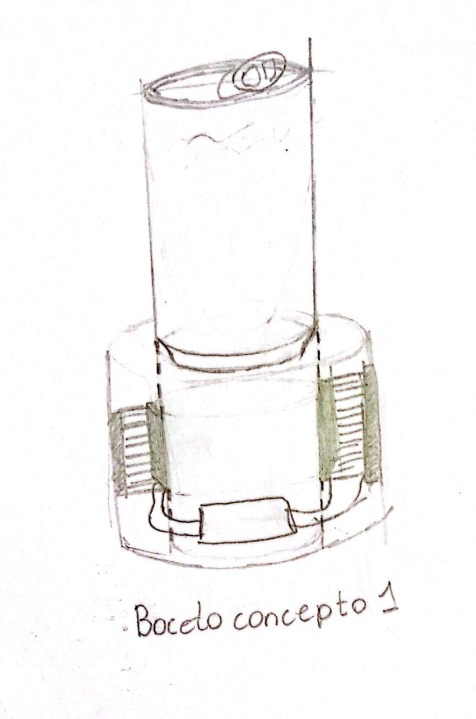
\includegraphics[width=\textwidth]{BC1.jpeg}
        \caption{Boceto 1: Manga conductiva.}
        \label{fig:boceto1}
    \end{subfigure}
    \hfill
    \begin{subfigure}[b]{0.45\textwidth}
        \centering
        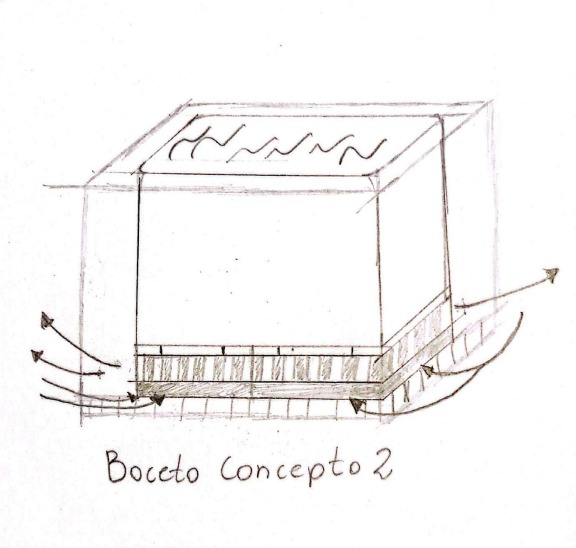
\includegraphics[width=\textwidth]{BC2.jpeg}
        \caption{Boceto 2: Baño líquido intermedio.}
        \label{fig:boceto2}
    \end{subfigure}
    
    \vspace{0.4cm}
    
    % Segunda fila: Boceto 3 y Boceto 4
    \begin{subfigure}[b]{0.45\textwidth}
        \centering
        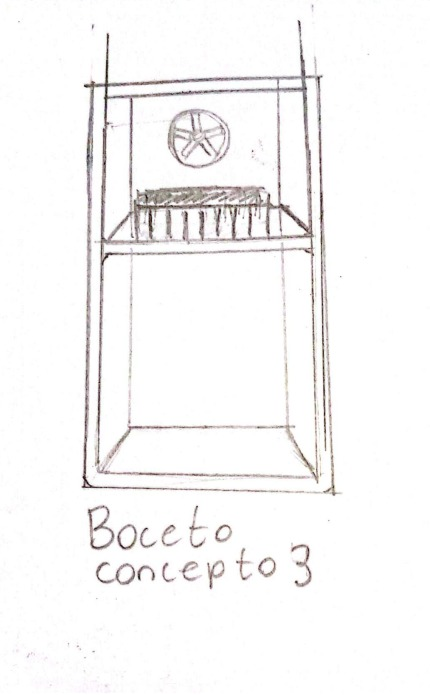
\includegraphics[width=\textwidth]{BC3.jpeg}
        \caption{Boceto 3: Cámara de aire.}
        \label{fig:boceto3}
    \end{subfigure}
    \hfill
    \begin{subfigure}[b]{0.45\textwidth}
        \centering
        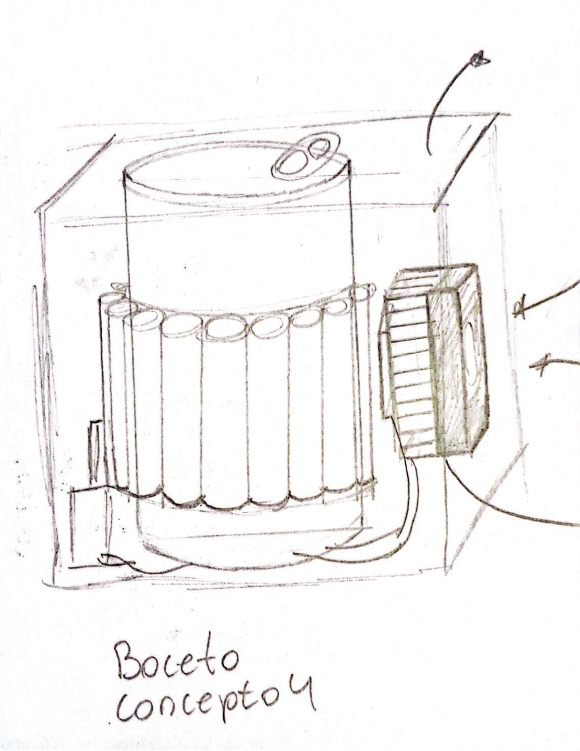
\includegraphics[width=\textwidth]{BC4.jpeg}
        \caption{Boceto 4: Lata rotatoria.}
        \label{fig:boceto4}
    \end{subfigure}
    
    \caption{Esquemas y bocetos de las alternativas de solución (parte 1).}
    \label{fig:bocetos_parte1}
\end{figure}

\clearpage % Fuerza a que el Boceto 5 pase limpio a la siguiente página

\begin{figure}[H]
    \centering
    % Tercera fila: Boceto 5 centrado en la siguiente página
    \begin{subfigure}[b]{0.45\textwidth}
        \centering
        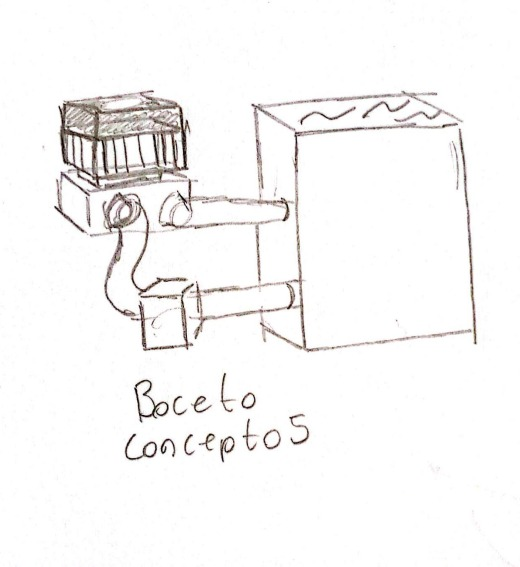
\includegraphics[width=\textwidth]{BC5.jpeg}
        \caption{Boceto 5: Bombeo conductivo.}
        \label{fig:boceto5}
    \end{subfigure}
    
    \caption{Esquemas y bocetos de las alternativas de solución (continuación).}
    \label{fig:bocetos_parte2}
\end{figure}
\subsubsection{Filtro de factibilidad}
Las alternativas se someten a un filtro para analizar si cumplen o no las restricciones. La Tabla \ref{tab:filtro} resume el resultado.

\begin{table}[H]
\centering
\small
\begin{tabular}{lccccc}
\toprule
\textbf{Restricción} & \textbf{C1} & \textbf{C2} & \textbf{C3} & \textbf{C4} & \textbf{C5} \\
\midrule
Opera en frío y calor con Peltier         & \cmark & \cmark & \cmark & \cmark & \cmark \\
Compatible con lata cerrada               & \cmark & \cmark & \cmark & \cmark & \cmark \\
Contacto alimentario garantizable         & \cmark & \cmark & \cmark & \cmark & \xmark \\ 
Fabricable mayormente por impresión 3D    & \cmark & \cmark & \cmark & \xmark & \xmark \\
Tiempos objetivo alcanzables              & \cmark & \cmark & \xmark & \cmark & \cmark \\ 
\midrule
\textbf{Resultado}                        & Cumple & Cumple & No Cumple & No Cumple & No Cumple \\
\bottomrule
\end{tabular}
\caption{Filtro de factibilidad de las alternativas frente a las restricciones.}
\label{tab:filtro}
\end{table}

El coeficiente de convección natural del aire es del orden de 5--25~\si{\watt\per\square\metre\per\kelvin} \parencite{incropera2007}, por lo que un concepto como C3 tiende a requerir tiempos del orden de horas, tal como se observa en el mini refrigerador AstroAI. El contacto conductivo y la convección en líquidos permiten coeficientes efectivos uno a dos órdenes de magnitud mayores \parencite{incropera2007}, acelerando la tasa de transferencia térmica hacia el volumen de la bebida.
En el caso del sistema de bombeo, al utilizar un sistema de bombas que en el contexto de placas Peltier están diseñadas mayormente para el bombeo de refrigerantes u otros fluidos no destinados al consumo humano \parencite{bomba_dc12v_2026}, al poseer partes móviles que desplazan el líquido, no se puede asegurar que se cumplan las normas sanitarias con las bombas disponibles en el mercado.

\subsubsection{Matriz de decisión ponderada}
Las alternativas que superan el filtro se evalúan en una escala de 1 a 5 frente a cada necesidad. Se suman las multiplicaciones de estos valores con los respectivos $P_j$ y se divide en 100. La Tabla \ref{tab:matriz_decision} presenta esto:

\begin{table}[H]
\centering
\small
\begin{tabular}{lccccc}
\toprule
\textbf{Necesidad} & $P_j$ & \textbf{C1} & \textbf{C2} \\
\midrule
Enfriamiento efectivo   & 16,7 & 3 & 4 \\
Calentamiento efectivo  & 15,3 & 4 & 4 \\
Tiempo de respuesta     & 12,2 & 3 & 4 \\
Facilidad de uso        & 7,3  & 4 & 4 \\
Limpieza e higiene      & 10,9 & 4 & 3 \\
Portabilidad            & 5,6  & 4 & 4 \\
Inocuidad               & 8,9  & 4 & 4 \\
Protección integral     & 10,5 & 4 & 3 \\
Bajo costo              & 6,7  & 4 & 4 \\
Eficiencia energética   & 5,8  & 3 & 3 \\
\midrule
\textbf{Puntaje ponderado} $U_a$ & 100 & \textbf{3,65} & \textbf{3,73} \\
\bottomrule
\end{tabular}
\caption{Matriz de decisión ponderada de las alternativas factibles.}
\label{tab:matriz_decision}
\end{table}

\subsubsection{Concepto seleccionado}
De acuerdo con la Tabla \ref{tab:matriz_decision}, el concepto seleccionado es el baño líquido intermedio (C2), con un puntaje ponderado de 3,73, frente a 3,65 de la manga conductiva (C1). Como ambas alternativas superan el filtro de factibilidad, la diferencia se explica por su desempeño en las necesidades de mayor peso. C2 obtiene una mejor evaluación en enfriamiento efectivo ($P_j = 16{,}7$) y en tiempo de respuesta ($P_j = 12{,}2$). Esto se debe a que el líquido envuelve por completo la superficie lateral de la lata y elimina la resistencia térmica de contacto entre la lata y la manga, la cual depende fuertemente de las tolerancias del diámetro de la lata y del ajuste de la pieza. También, el baño distribuye el calor de forma uniforme sobre la carga, mientras que en la manga conductiva resulta difícil lograr un calentamiento homogéneo.

Sin embargo, C2 obtiene una menor evaluación en limpieza e higiene y en protección integral, ya que el depósito de fluido introduce riesgos de derrame, condensación y mantenimiento del fluido de trabajo que no existen en la manga. En modo frío, el fluido debe preenfriarse antes de lograr una transferencia eficaz, lo que no ocurre con la manga; en modo calor, el fluido debe elevarse por sobre \SI{85}{\celsius}, lo que aumenta la energía requerida y afecta al tiempo objetivo de calentamiento. Estos problemas se abordarán en las etapas siguientes considerando:

\begin{itemize}
    \item El volumen de fluido de trabajo se dimensionará mediante el modelo térmico transitorio, buscando el mínimo volumen que asegure el contacto completo con la lata y con el recipiente, de modo de reducir la masa térmica del sistema.
    \item El modelo termoeléctrico evaluará la operación de los módulos Peltier con el fluido a temperaturas cercanas a \SI{90}{\celsius}, verificando que la diferencia de temperatura resultante se mantenga dentro de los límites del kit.
    \item El diseño mecánico considerará un depósito sellado con tapa, aislamiento térmico y una bandeja colectora de condensado y derrames.
\end{itemize}

En cuanto a la inocuidad, la manga conductiva ofrece la ventaja de que ningún componente del equipo entra en contacto con el agua de consumo. Esta característica se incorpora al concepto seleccionado, dando lugar a una solución híbrida: el agua de consumo se calienta dentro de un recipiente removible de acero inoxidable AISI~304 sumergido en el baño, de modo que nunca entra en contacto con el fluido de trabajo, mientras que la lata se enfría cerrada dentro del mismo baño. Adicionalmente, se explorarán soluciones intermedias, como una camisa conductiva por la que circule el fluido de trabajo, siempre que se mantenga separado del agua de consumo.

Cabe destacar que la diferencia entre ambas alternativas es reducida (0,08 puntos). La ventaja de C2 en enfriamiento y tiempo de respuesta deberá confirmarse mediante el modelo térmico transitorio desarrollado en la Sección \ref{sec:simulaciones}. Si no se confirma la ventaja, se evaluará considerar la manga conductiva.

Finalmente, al comparar con los productos de referencia de la Tabla \ref{tab:competencia_necesidades}, el concepto seleccionado supera a todos los productos de doble modo, como el portavasos termoeléctrico (3,38) y el mini refrigerador AstroAI (2,62), y también a los enfriadores rápidos Cooper Cooler (3,26) y SpinChill (3,57). Solo el hervidor eléctrico alcanza un puntaje levemente superior (3,74), resultado esperable al tratarse de un producto especializado en una única función. Cabe mencionar que el puntaje de C2 corresponde a la evaluación de un concepto y no de un producto terminado, por lo que deberá verificarse con el prototipo que se fabricará en el Desafío 3.


\section{Arquitectura y modelos desarrollados}

\section{Simulaciones y justificación físico-matemática}
\label{sec:simulaciones}

\section{Caracterización, calibración y validación inicial}

\section{Desarrollo del producto final y plan de fabricación}

\section{Resultados y discusión}

\section{Conclusiones}

% ------------------------------------------
% BIBLIOGRAFÍA
% ------------------------------------------
\newpage
\nocite{*}
\printbibliography[heading=bibintoc, title={Referencias Bibliográficas}]

\end{document}